\documentclass{beamer}
\usepackage{listings}
\usepackage{hyperref}
\usepackage{tikz}
\usetikzlibrary{positioning,shadows,arrows,shapes,calc}
\usepackage{amsmath}
\newcommand{\argmax}{\operatornamewithlimits{argmax}}
\newcommand{\softmax}{\operatornamewithlimits{softmax}}
\def\labelenumi\theenumi
\usepackage{graphicx}
\mode<presentation>{\usetheme{Frankfurt}}
\AtBeginSection
{
  \begin{frame}<beamer>
    \frametitle{Outline}
    \tableofcontents[currentsection,currentsubsection]
  \end{frame}
}
\title{Lecture 26: Final Exam Review, Part 1}
\author{Mark Hasegawa-Johnson}
\date{ECE 417: Multimedia Signal Processing}
\institute{University of Illinois}
\titlegraphic{\includegraphics{../../images/imark_1867_bold.png}}
\begin{document}

% Title
\begin{frame}
  \maketitle
\end{frame}

% Title
\begin{frame}
  \tableofcontents
\end{frame}


%%%%%%%%%%%%%%%%%%%%%%%%%%%%%%%%%%%%%%%%%%%%%%%%%%%%%%%%%
\section{Topics}
\setcounter{subsection}{1}

\begin{frame}
  \frametitle{Final Exam: General Structure}

  \begin{itemize}
  \item About twice as long as a midterm (i.e., 8-10 problems with 1-3 parts each)
  \item You'll have 3 hours for the exam (December 13, 8-11am)
  \item The usual rules: no calculators or computers, two sheets of
    handwritten notes, you will have two pages of formulas provided on
    the exam, published by the Friday before the exam.  
  \end{itemize}
\end{frame}

\begin{frame}
  \frametitle{Final Exam: Topics Covered}

  \begin{itemize}
  \item 17\%: Material from exam 1 (signal processing)
  \item 17\%: Material from exam 2 (probability)
  \item 66\%: Material from the last third of the course (neural networks)
  \end{itemize}
\end{frame}

\begin{frame}
  \frametitle{Material from the last third of the course}

  \begin{itemize}
  \item Neural networks \& back-propagation
  \item CNN \& Faster RCNN
  \item Partial derivatives \& RNN
  \item LSTM
  \end{itemize}
\end{frame}

%%%%%%%%%%%%%%%%%%%%%%%%%%%%%%%%%%%%%%%%%%%%%%%%%%%%%%%%%
\section{Neural Networks}
\setcounter{subsection}{1}

\begin{frame}
  \frametitle{Two-Layer Feedforward Neural Network}
  \begin{small}
      \begin{center}
        \tikzstyle{pre}=[<-,shorten <=1pt,>=stealth',semithick,draw=blue]
        \tikzstyle{post}=[->,shorten >=1pt,>=stealth',semithick,draw=blue]
        \begin{tikzpicture}[
            hoop/.style={circle,thick, draw=blue, text=black, fill=orange!35!white, text centered, text width=0.25cm},
            open/.style={circle,thick, draw=blue, text=black, text centered, text width=0.25cm}
          ]
          \node (x0) at (0,0) {$1$};
          \node[open] (x1) at (1,0) {$x_1$};
          \node[open] (x2) at (2,0) {$x_2$};
          \node (x3) at (3,0) {\ldots};
          \node[open] (xp) at (4,0) {$x_D$};
          \node (input) at (7,0) {$\vec{x}$ is the input vector};
          \node (e1sum) at (7,0.75) {$\xi_k^{(1)} = b_{k}^{(1)}+\sum_{j=1}^Dw_{kj}^{(1)}x_j$};
          %\node (e1vec) at (9,0.75) {$\vec{e}^{(1)}=W^{(1)}\vec{x}+\vec{b}^{(1)}$};
          \node (h0) at (0,1.5) {$1$};
          \node[hoop] (h1) at (1,1.5) {$h_1$} edge[pre](x0) edge[pre](x1) edge[pre](xp);
          \node[hoop] (h2) at (2,1.5) {$h_2$} edge[pre](x0) edge[pre](x1) edge[pre](xp);
          \node (y3) at (3,1.5) {\ldots};
          \node[hoop] (hq) at (4,1.5) {$h_N$} edge[pre](x0) edge[pre](x1) edge[pre](xp);
          \node (hsum) at (7,1.5) {$h_k=g(\xi_k^{(1)})$};
          %\node (hvec) at (9,1.5) {$\vec{h}=f(\vec{e}^{(1)})$};
          \node (e2sum) at (7,2.25) {$\xi_k^{(2)}=b_{k}^{(2)}+\sum_{j=1}^N w_{kj}^{(2)}h_j$};
          %\node (e2vec) at (9,2.25) {$\vec{e}^{(2)}=W^{(2)}\vec{h}+\vec{b}^{(2)}$};
          \node[hoop] (y1) at (1,3) {$\hat{y}_1$} edge[pre](h0) edge[pre](h1) edge[pre](hq);
          \node[hoop] (y2) at (2,3) {$\hat{y}_2$} edge[pre](h0) edge[pre](h1) edge[pre](hq);
          \node (y3) at (3,3) {\ldots};
          \node[hoop] (yr) at (4,3) {$\hat{y}_K$} edge[pre](h0) edge[pre](h1) edge[pre](hq);
          \node (ysum) at (7,3) {$\hat{y}_k=g(\xi_k^{(2)})$};
          %\node (yvec) at (9,3) {$\hat{y}=\vec{e}^{(2)}$};
          \node (zeta1) at (1,3.75) {} edge[pre](y1);
          \node (zeta2) at (2,3.75) {} edge[pre](y2);
          \node (zetar) at (4,3.75) {} edge[pre](yr);
          \node (output) at (2.5,4) {$\hat{y}=h(\vec{x},W^{(1)},\vec{b}^{(1)},W^{(2)},\vec{b}^{(2)})$};
        \end{tikzpicture}
      \end{center}
  \end{small}
\end{frame}

\begin{frame}
  \frametitle{How to train a neural network}
  \begin{enumerate}
  \item Find a {\bf training dataset} that contains $n$ examples showing the
    desired output, $\vec{y}_i$, that the NN should compute in
    response to input vector $\vec{x}_i$:
    \[
    {\mathcal D}=\left\{(\vec{x}_1,\vec{y}_1),\ldots,(\vec{x}_n,\vec{y}_n)\right\}
    \]
    \item Randomly {\bf initialize} $W^{(1)}$,
      $\vec{b}^{(1)}$, $W^{(2)}$, and $\vec{b}^{(2)}$.
    \item Perform {\bf forward propagation}: find out what the neural
      net computes as $\hat{y}_i$ for each $\vec{x}_i$.
    \item Define a {\bf loss function} that measures
      how badly $\hat{y}$ differs from $\vec{y}$.
    \item Perform {\bf back propagation} to find the derivative of the loss w.r.t.  $W^{(1)}$,
      $\vec{b}^{(1)}$, $W^{(2)}$, and $\vec{b}^{(2)}$.
    \item Perform {\bf gradient descent} to improve  $W^{(1)}$,
      $\vec{b}^{(1)}$, $W^{(2)}$, and $\vec{b}^{(2)}$.
    \item Repeat steps 3-6 until convergence.
  \end{enumerate}
\end{frame}

\begin{frame}
\begin{block}{Gradient Descent = Local Optimization}
  Given an initial $W,b$, find new values of $W$, $b$ with lower error.
  \begin{align*}
    w_{kj}^{(1)} &\leftarrow w_{kj}^{(1)}-\eta\frac{d{\mathcal L}}{d w_{kj}^{(1)}}\\
    w_{kj}^{(2)} &\leftarrow w_{kj}^{(2)}-\eta\frac{d{\mathcal L}}{d w_{kj}^{(2)}}
  \end{align*}
\end{block}
\begin{block}{$\eta=$Learning Rate}
    \begin{itemize}
      \item If $\eta$ too large, gradient descent won't converge. If
        too small, convergence is slow.
      \item Second-order methods like Newton's method, L-BFGS and Adam choose an optimal $\eta$
        at each step, so they're MUCH faster.
    \end{itemize}
\end{block}
\end{frame}

\begin{frame}
  \frametitle{Loss Function: How should $y$ be
    ``similar to'' $\hat{y}$?}
  \begin{block}{Minimum Mean Squared Error (MMSE)}
    \[
    W^*,b^*=\arg\min {\mathcal L} = \arg\min\frac{1}{2n}\sum_{i=1}^n
    \Vert\vec{y}_{i}-\hat{y}(\vec{x}_i)\Vert^2
    \]
  \end{block}
  \begin{block}{MMSE Solution: $\hat{y}\rightarrow E\left[\vec{y}|\vec{x}\right]$}
    If the training samples $(\vec{x}_i,\vec{y}_i)$ are i.i.d., then
    \[
    \lim_{n\rightarrow\infty}{\mathcal L} = \frac{1}{2}E\left[\Vert\vec{y}-\hat{y}\Vert^2\right]
    \]
    which is minimized by
    \[
    \hat{y}_{MMSE}(\vec{x})=E\left[\vec{y}|\vec{x}\right]
    \]
  \end{block}
\end{frame}

\begin{frame}
  \frametitle{Binary Cross Entropy}

  Suppose we treat the neural net output as a noisy
  estimator, $\hat{p}_{Y|\vec{X}}(y|\vec{x})$, of the unknown true pmf
  $p_{Y|\vec{X}}\left(y|\vec{x}\right)$:
  \[
  \hat{y}_i = \hat{p}_{Y|\vec{X}}(1|\vec{x}),
  \]
  so that
  \begin{displaymath}
    \hat{p}_{Y|\vec{X}}(y_i|\vec{x}_i)
    =\begin{cases}\hat{y}_i & y_i=1\\1-\hat{y}_i & y_i=0\end{cases}
  \end{displaymath}
  The binary cross-entropy loss is the negative log probability of the
  training data, assuming i.i.d. training examples:
  \begin{align*}
    {\mathcal L}_{BCE} &= -\frac{1}{n}\sum_{i=1}^n \ln\hat{p}_{Y|\vec{X}}(y_i|\vec{x}_i)\\
    &= -\frac{1}{n}\sum_{i=1}^n
    y_i\left(\ln\hat{y}_i\right)+
    (1-y_i)\left(\ln(1-\hat{y}_i)\right)
  \end{align*}
\end{frame}

\begin{frame}
  \frametitle{The Derivative of BCE}

  BCE is useful because it has the same solution as MSE, without
  allowing the sigmoid to suffer from vanishing gradients.  Suppose
  $\hat{y}_i=\sigma(\xi_i)$.
  \begin{align*}
    \frac{\partial{\mathcal L}}{\partial\xi_i}
    &=
    -\frac{1}{n}
    \left(y_i\frac{\partial\ln\sigma(\xi_i)}{\partial\xi_i}
    +(1-y_i)\frac{\partial\ln(1-\sigma(\xi_i))}{\partial\xi_i}\right)\\
    &=
    -\frac{1}{n}
    \left(y_i\frac{\dot\sigma(\xi_i)}{\sigma(\xi_i)}-
    (1-y_i)\frac{1-\dot\sigma(\xi_i)}{1-\sigma(\xi_i)}\right)\\
    &=
    -\frac{1}{n}
    \left(y_i\frac{\hat{y}_i(1-\hat{y}_i)}{\hat{y}_i}
    -(1-y_i)\frac{\hat{y}_i(1-\hat{y}_i)}{1-\hat{y}_i}
    \right)\\
    &=
    -\frac{1}{n}
    \left(y_i-\hat{y}_i\right)
  \end{align*}
  where the last line is true because $y_i\in\{0,1\}$.
\end{frame}

\begin{frame}
  \frametitle{Multinomial Classifier}

  Suppose, instead of just a 2-class classifier, we want the neural
  network to classify $\vec{x}$ as being one of $K$ different classes.
  There are many ways to encode this, but one of the best is
  \begin{displaymath}
    \vec{y}=\left[\begin{array}{c}y_1\\y_2\\\vdots\\y_K\end{array}\right],~~~
    y_k=\begin{cases}1&k=k^*~~(k~\mbox{is the correct class})\\0&\mbox{otherwise}\end{cases}
  \end{displaymath}
  A vector $\vec{y}$ like this is called a ``one-hot vector,'' because
  it is a binary vector in which only one of the elements is nonzero (``hot'').
  This is useful  because minimizing the MSE loss gives:
  \begin{displaymath}
    \hat{y}=\left[\begin{array}{c}\hat{y}_1\\\hat{y}_2\\\vdots\\\hat{y}_K\end{array}\right]
    =\left[\begin{array}{c}
        \hat{p}_{Y_1|\vec{X}}(1|\vec{x})\\
        \hat{p}_{Y_2|\vec{X}}(1|\vec{x})\\
        \vdots\\
        \hat{p}_{Y_K|\vec{X}}(1|\vec{x})
        \end{array}\right],
  \end{displaymath}
  where the global optimum of
  $\hat{p}_{Y_k|\vec{X}}(y|\vec{x})\rightarrow
  p_{Y_k|\vec{X}}(y|\vec{x})$ as $n\rightarrow\infty$.
\end{frame}

\begin{frame}
  \frametitle{One-hot vectors and Cross-entropy loss}
  
  The cross-entropy loss, for a training database coded with one-hot vectors, is
  \begin{align*}
    {\mathcal L}_{CE} &=-\frac{1}{n}\sum_{i=1}^n\sum_{k=1}^K y_{ki}\ln\hat{y}_{ki}
  \end{align*}
  This is useful because:
  \begin{enumerate}
  \item {\bf Like MSE, Cross-Entropy has an asymptotic global optimum at:}
    $\hat{y}_k\rightarrow p_{Y_k|\vec{X}}(1|\vec{x})$.
  \item {\bf Unlike MSE, Cross-Entropy with a softmax nonlinearity
    suffers no vanishing gradient problem.}
  \end{enumerate}
\end{frame}

\begin{frame}
  \frametitle{Softmax Nonlinearity}

  The multinomial cross-entropy loss is only well-defined if
  $0<\hat{y}_{ki}<1$, and it is only well-interpretable if
  $\sum_k\hat{y}_{ki}=1$.  We can guarantee these two properties by
  setting
  \begin{align*}
    \hat{y}_k &= \softmax_k\left(W\vec{h}\right)\\
    &= \frac{\exp(\bar{w}_k\vec{h})}{\sum_{\ell=1}^K
      \exp(\bar{w}_\ell\vec{h})},
  \end{align*}
  where $\bar{w}_k$ is the $k^{\textrm{th}}$ row of the $W$ matrix.
\end{frame}

\begin{frame}
  \frametitle{Sigmoid is a special case of Softmax!}

  \begin{displaymath}
    \softmax_k\left(W\vec{h}\right)
    = \frac{\exp(\bar{w}_k\vec{h})}{\sum_{\ell=1}^K
      \exp(\bar{w}_\ell\vec{h})}.
  \end{displaymath}
  Notice that, in the 2-class case, the softmax is just exactly a
  logistic sigmoid function:
  \begin{displaymath}
    \softmax_1(W\vec{h}) = \frac{e^{\bar{w}_1\vec{h}}}{e^{\bar{w}_1\vec{h}}+e^{\bar{w}_2\vec{h}}}
    = \frac{1}{1+e^{-(\bar{w}_1-\bar{w}_2)\vec{h}}}  =\sigma\left((\bar{w}_1-\bar{w}_2)\vec{h}\right)
  \end{displaymath}
  so everything that you've already learned about the sigmoid applies
  equally well here.
\end{frame}

\begin{frame}
  \frametitle{The Total Derivative Rule}

  The {\bf total derivative rule} says that the derivative of the
  output with respect to any one input can be computed as the sum of
  partial times total, summed across all paths from input to output:

  \begin{displaymath}
    \frac{\partial y(x,z)}{\partial x} =
    \left(\frac{d y}{d g}\right)\left(\frac{\partial g(x,z)}{\partial x}\right) +
    \left(\frac{d y}{d h}\right)\left(\frac{\partial h(g,x,z)}{\partial x}\right)
  \end{displaymath}

  \begin{center}
    \tikzstyle{pre}=[<-,shorten <=1pt,>=stealth',semithick,draw=blue]
    \tikzstyle{post}=[->,shorten >=1pt,>=stealth',semithick,draw=blue]
    \begin{tikzpicture}[
        hoop/.style={circle,thick, draw=blue, text=black, fill=orange!35!white, text centered, text width=0.25cm},
        open/.style={circle,thick, draw=blue, text=black, text centered, text width=0.25cm}
      ]
      \node[open] (x) at (0,-1) {$x$};
      \node[open] (z) at (0,1) {$z$} edge[pre](x);
      \draw[dashed] (1,-1.5) -- (1,1.5);
      \node[open] (g) at (2,-1) {$g$} edge[pre](x) edge[pre](z);
      \node[open] (h) at (2,1) {$h$} edge[pre](x) edge[pre](z) edge[pre](g);
      \node[open] (u) at (4,-1) {$u$} edge[pre](g) edge[pre](h);
      \node[open] (v) at (4,1) {$v$} edge[pre](g) edge[pre](h);
      \node[open] (y) at (6,0) {$y$} edge[pre](u) edge[pre](v);
    \end{tikzpicture}
  \end{center}
\end{frame}

\begin{frame}
  \begin{block}{The Back-Propagation Algorithm}
    \[
    W^{(2)}\leftarrow W^{(2)}-\eta\nabla_{W^{(2)}}{\mathcal L},~~~~~
    W^{(1)}\leftarrow W^{(1)}-\eta\nabla_{W^{(1)}}{\mathcal L}
    \]
    \[
    \nabla_{W^{(2)}}{\mathcal L}=\sum_{i=1}^n \nabla_{\vec\xi_i^{(2)}}{\mathcal L}
    \vec{h}_i^T,~~~~~
    \nabla_{W^{(1)}}{\mathcal L}=\sum_{i=1}^n\nabla_{\vec\xi_i^{(1)}}{\mathcal L}
    \vec{x}_i^T
    \]
    \[
    \nabla_{\vec\xi_i^{(2)}}{\mathcal L}=\frac{1}{n} (\hat{y}_{i}-\vec{y}_{i}),~~~~~
    \nabla_{\vec\xi_i^{(1)}}{\mathcal L}=\dot\sigma(\vec\xi_{i}^{(1)})\odot
    W^{(2),T}\nabla_{\vec\xi_i^{(2)}}{\mathcal L}
    \]
  \end{block}
\end{frame}

\begin{frame}
  \frametitle{Derivative of a sigmoid}
  The derivative of a sigmoid is pretty easy to calculate:
  \[
  h=\sigma(\xi)=\frac{1}{1+e^{-\xi}},~~~\frac{dh}{d\xi}=\dot\sigma(\xi)=\frac{e^{-\xi}}{(1+e^{-\xi})^2}
  \]
  An interesting fact that's extremely useful, in computing back-prop,
  is that if $h=\sigma(\xi)$, then we can write the derivative in terms
  of $h$, without any need to store $\xi$:
  \begin{align*}
    \frac{d\sigma}{d\xi} &=\frac{e^{-\xi}}{(1+e^{-\xi})^2}\\
    &=\left(\frac{1}{1+e^{-\xi}}\right)\left(\frac{e^{-\xi}}{1+e^{-\xi}}\right)\\
    &=\left(\frac{1}{1+e^{-\xi}}\right)\left(1-\frac{1}{1+e^{-\xi}}\right)\\
    &=\sigma(\xi)(1-\sigma(\xi))\\
    &=h(1-h)\\
  \end{align*}
\end{frame}

\begin{frame}
  \begin{columns}[t]
    \column{2.25in}
    \begin{block}{Step function and its derivative}
      \centerline{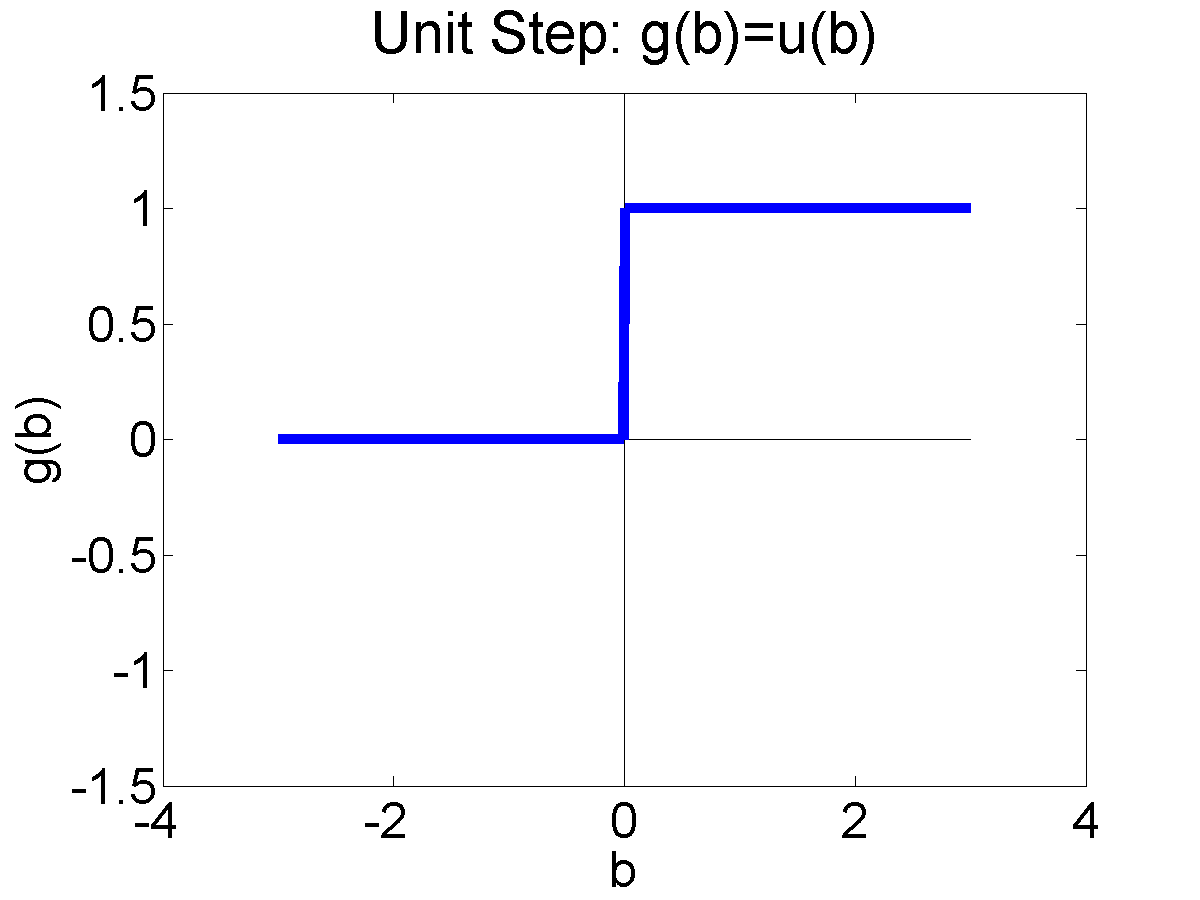
\includegraphics[width=1.75in]{figs/nn_unitstep.png}}
      \begin{itemize}
      \item The derivative of the step function is the Dirac
        delta, which is not very useful in backprop.
      \end{itemize}
    \end{block}
    \column{2.25in}
    \begin{block}{Logistic function and its derivative}
      \centerline{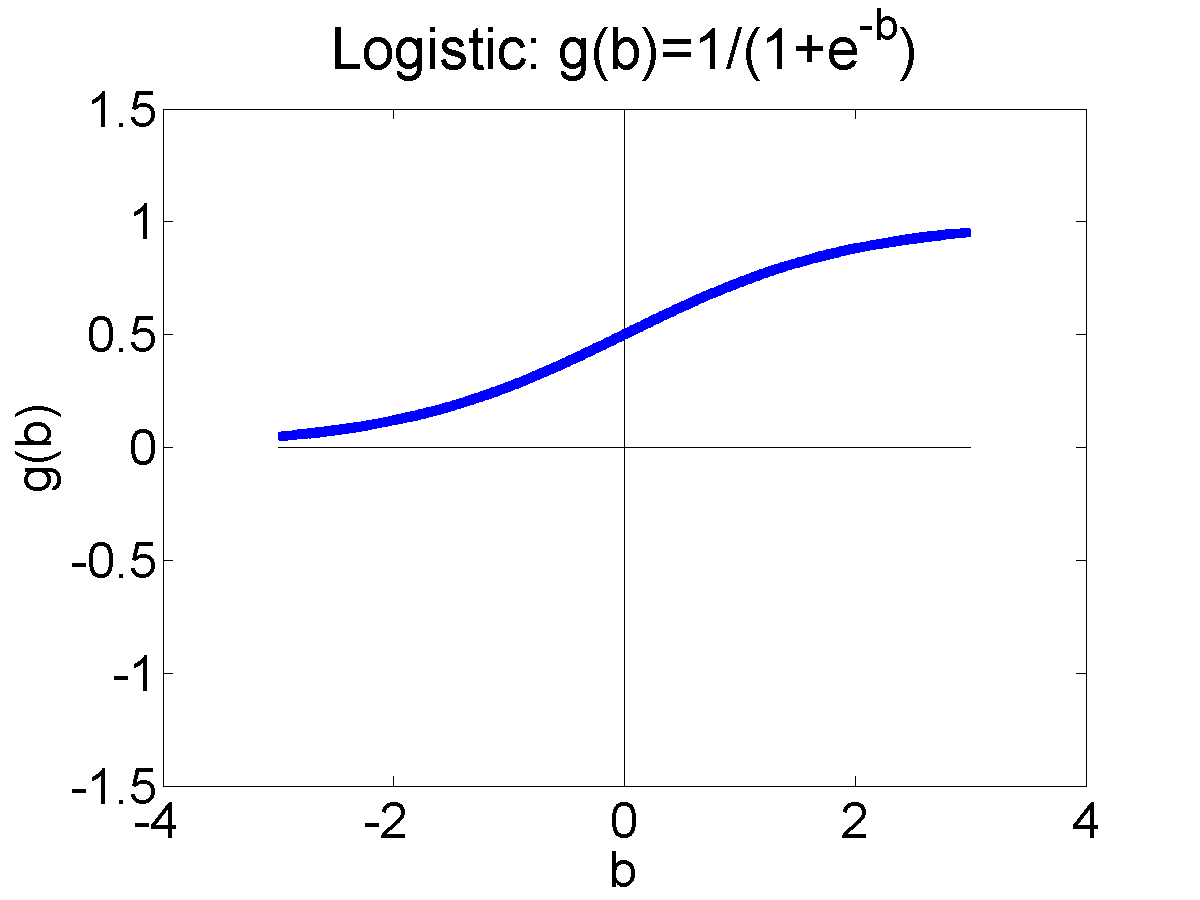
\includegraphics[width=1.75in]{figs/nn_logistic.png}}
      \centerline{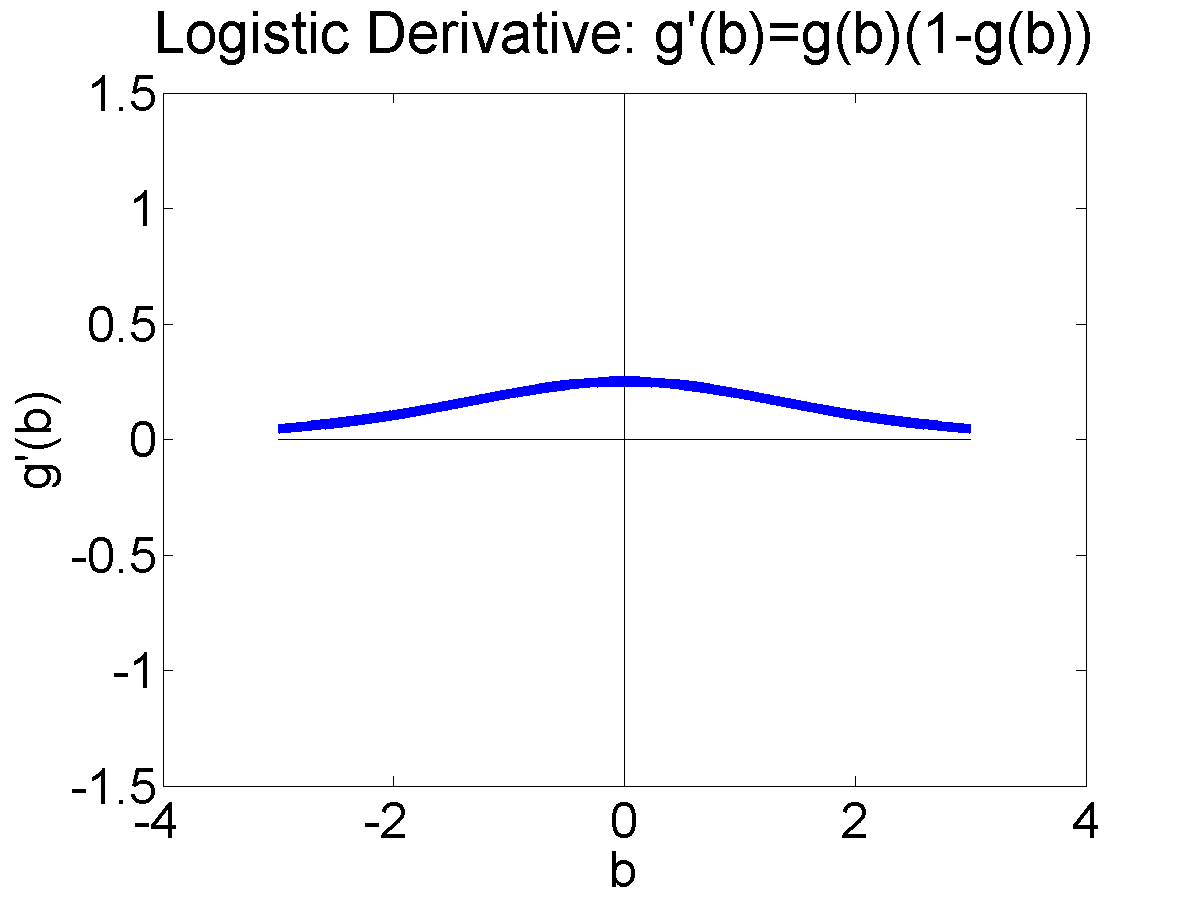
\includegraphics[width=1.75in]{figs/nn_logisticprime.png}}
    \end{block}
  \end{columns}
\end{frame}

\begin{frame}
  \frametitle{Signum and Tanh}

  The signum function is a signed binary nonlinearity.  It is used if,
  for some reason, you want your output to be
  $h\in\left\{-1,1\right\}$, instead of $h\in\left\{0,1\right\}$:
  \[
  \mbox{sign}(b)=\begin{cases}
  -1 & b<0\\
  1 & b>0
  \end{cases}
  \]
  It is usually approximated by the hyperbolic tangent function
  (tanh), which is just a scaled shifted version of the sigmoid:
  \begin{displaymath}
    h=\tanh(\xi) = \frac{e^\xi-e^{-\xi}}{e^\xi+e^{-\xi}}
    = \frac{1-e^{-2\xi}}{1+e^{-2\xi}}
    = 2\sigma(2\xi)-1
  \end{displaymath}
  and which has a scaled version of the sigmoid derivative:
  \begin{align*}
    \frac{d\tanh(\xi)}{d\xi} =\left(1-\tanh^2(\xi)\right)
  \end{align*}
\end{frame}

\begin{frame}
  \begin{columns}[t]
    \column{2.25in}
    \begin{block}{Signum function and its derivative}
      \centerline{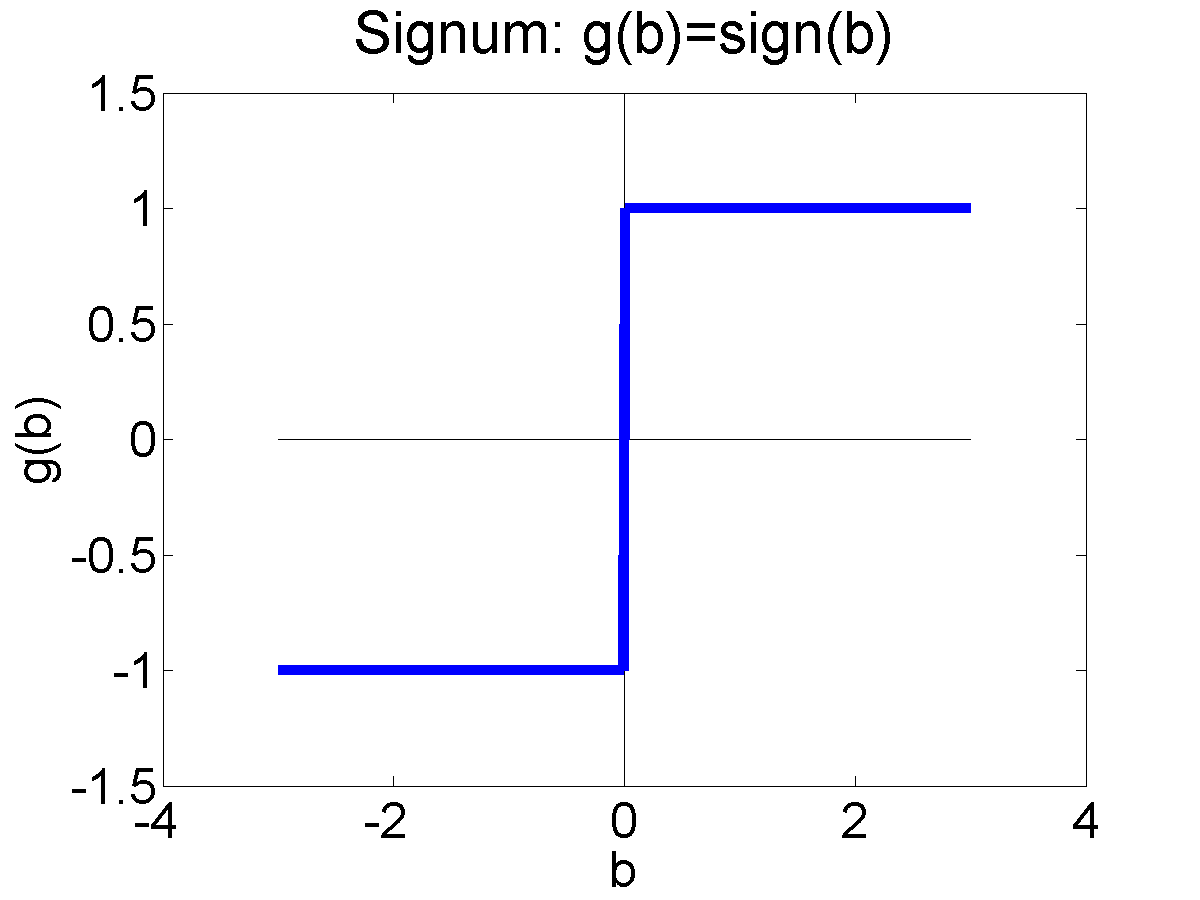
\includegraphics[width=1.75in]{figs/nn_signum.png}}
      \begin{itemize}
      \item The derivative of the signum function is the Dirac
        delta, which is not very useful in backprop.
      \end{itemize}
    \end{block}
    \column{2.25in}
    \begin{block}{Tanh function and its derivative}
      \centerline{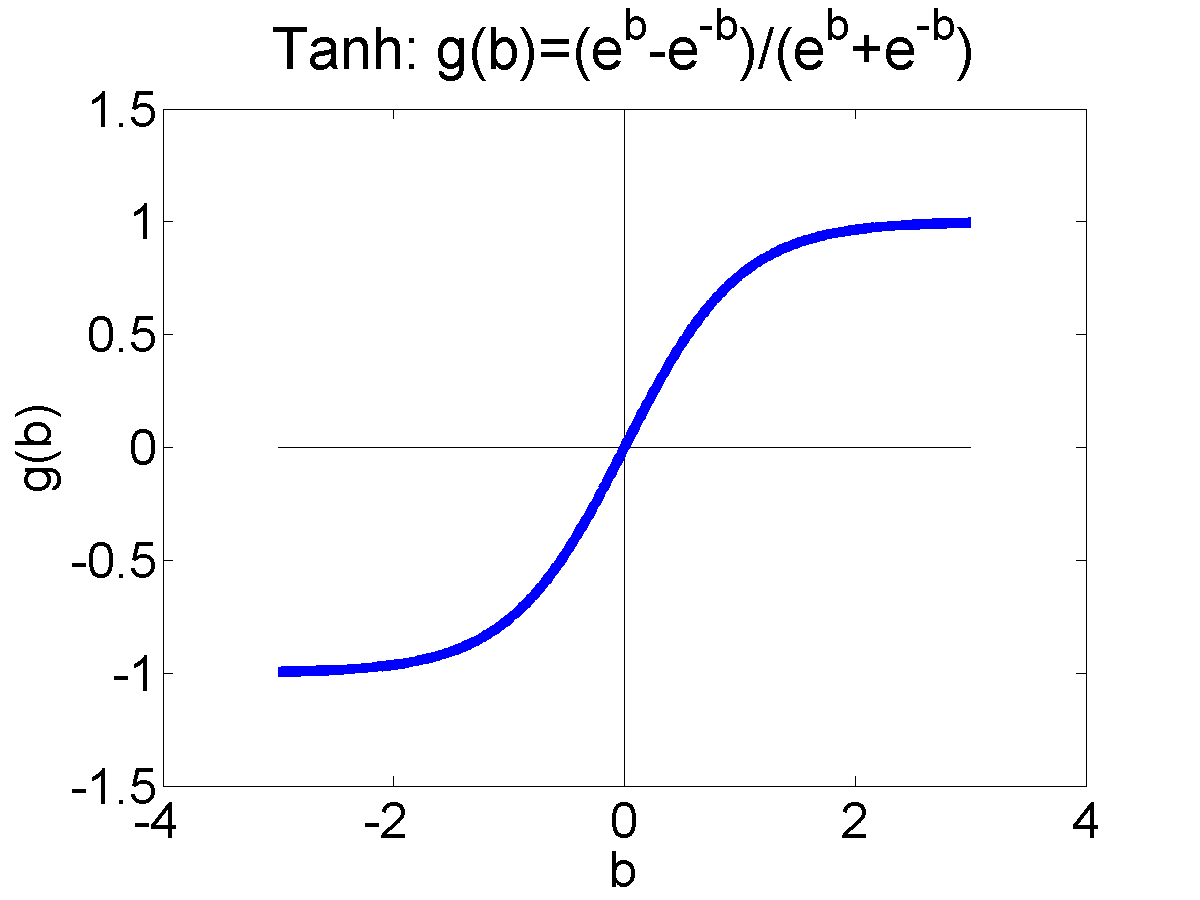
\includegraphics[width=1.75in]{figs/nn_tanh.png}}
      \centerline{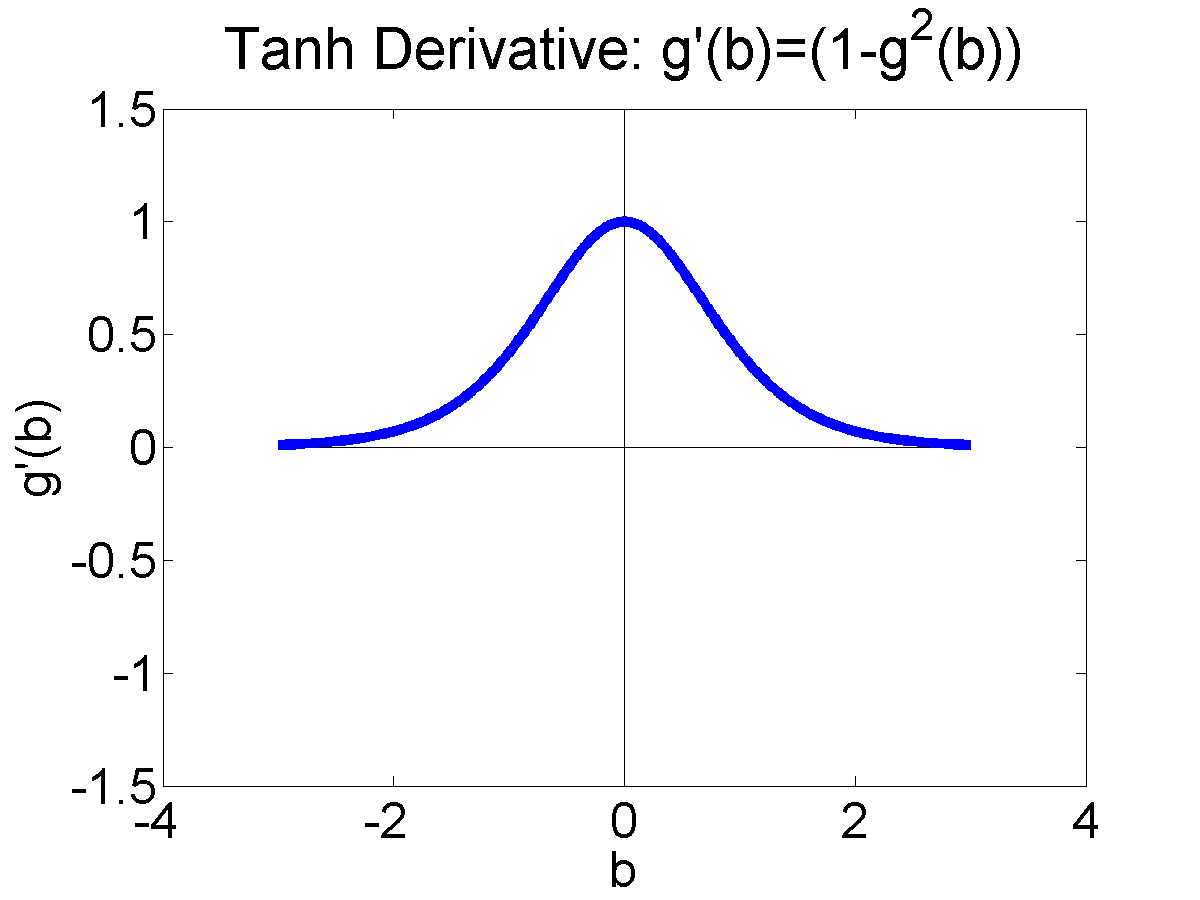
\includegraphics[width=1.75in]{figs/nn_tanhprime.png}}
    \end{block}
  \end{columns}
\end{frame}

\begin{frame}
  \frametitle{A solution to the vanishing gradient problem: ReLU}
  \centerline{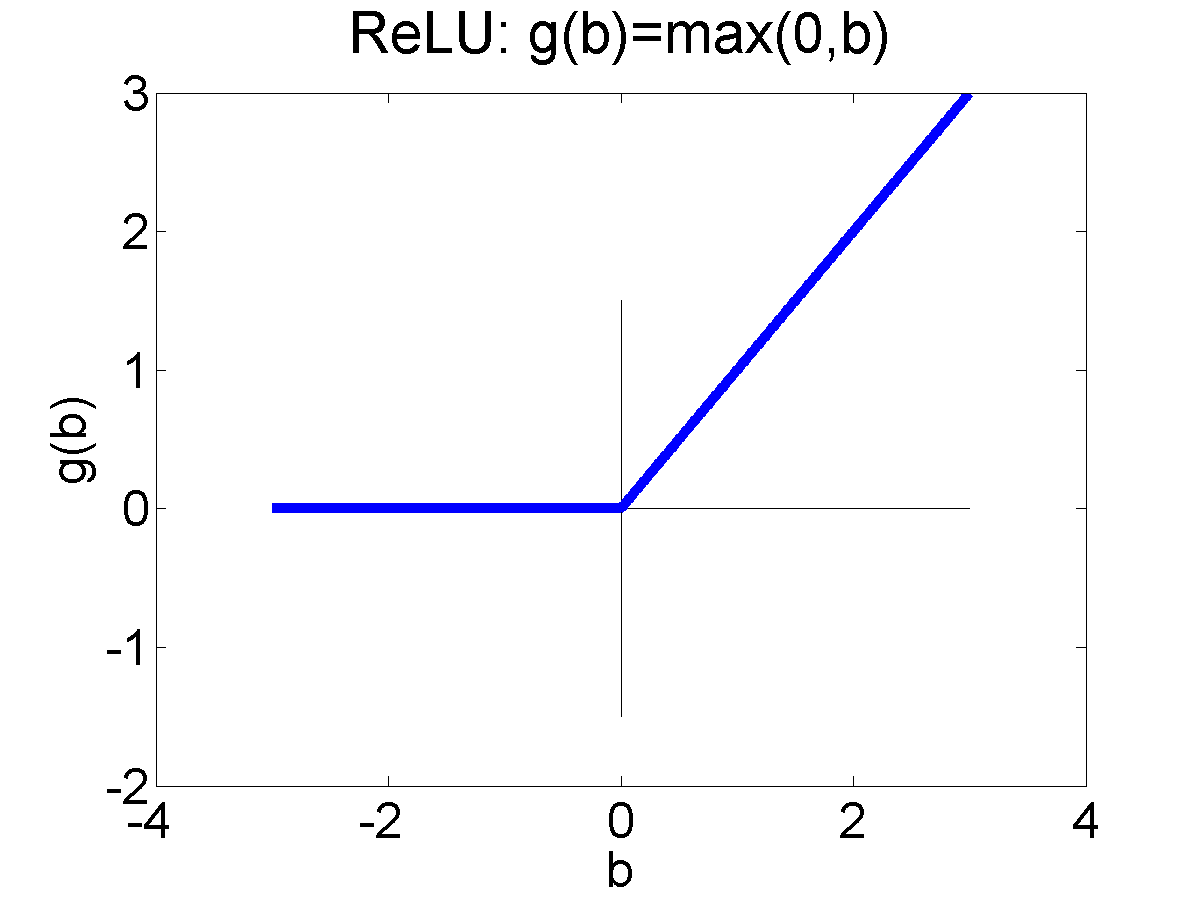
\includegraphics[width=1in]{figs/nn_relu.png}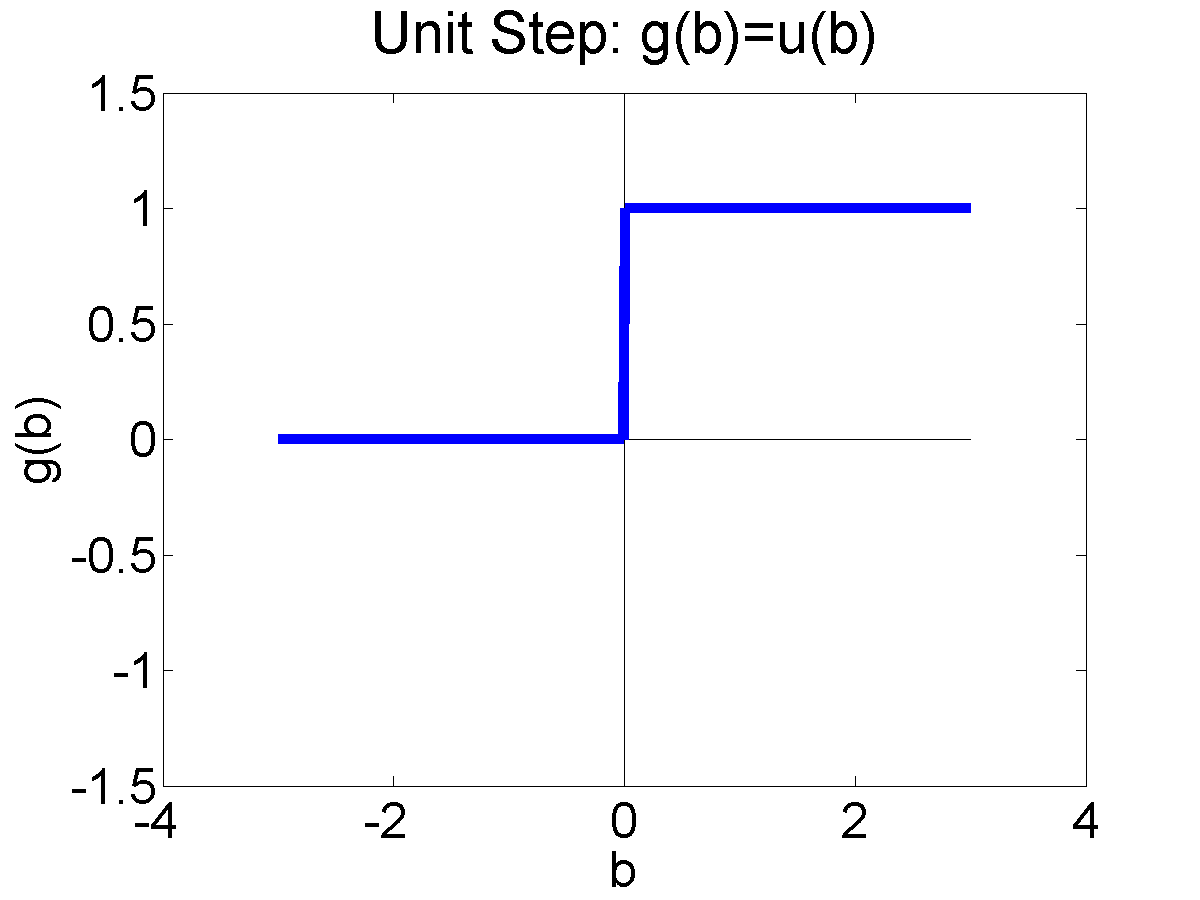
\includegraphics[width=1in]{figs/nn_unitstep.png}}

  The most ubiquitous solution to the vanishing gradient problem is to
  use a ReLU (rectified linear unit) instead of a sigmoid.  The ReLU
  is given by
  \[
  \mbox{ReLU}(\xi) = \begin{cases}
    b & \xi\ge 0\\
    0 & \xi\le 0,
  \end{cases}
  \]
  and its derivative is
  \[
  \frac{d\mbox{ReLU}(\xi)}{d(\xi)}=u(\xi)
  \]
\end{frame}

%%%%%%%%%%%%%%%%%%%%%%%%%%%%%%%%%%%%%%%%%%%%%%%%%%%%%%%%%
\section{CNN \& Faster-RCNN}
\setcounter{subsection}{1}

\begin{frame}
  \frametitle{How to achieve shift invariance: Convolution}

  Instead of using vectors as layers, let's use images.
  \begin{align*}
    \xi^{(l)}[m,n,d] &= \sum_c\sum_{m'}\sum_{n'} w^{(l)}[m',n',c,d]h^{(l-1)}[m-m',n-n',c]
  \end{align*}
  where
  \begin{itemize}
  \item $\xi^{(l)}[m,n,c]$ and $h^{(l)}[m,n,c]$ are excitation and
    activation (respectively) of the $(m,n)^{\textrm{th}}$ pixel, in
    the $c^{\textrm{th}}$ channel, in the $l^{\textrm{th}}$ layer.
  \item $w^{(l)}[m,n,c,d]$ are weights connecting $c^{\textrm{th}}$
    input channel to $d^{\textrm{th}}$ output channel, with a shift of
    $m$ rows, $n$ column.
  \end{itemize}
\end{frame}

\begin{frame}
  \frametitle{Convolution forward, Correlation backward}

  In signal processing, we defined $x[n]\ast h[n]$ to mean $\sum
  h[m]x[n-m]$.  Let's use the same symbol to refer to this
  multi-channel 2D convolution:
  \begin{align*}
    \xi^{(l)}[m,n,d] &= \sum_c\sum_{m'}\sum_{n'} w^{(l)}[m-m',n-n',c,d]h^{(l-1)}[m',n',c]\\
    &\equiv w^{(l)}[m,n,c,d] \ast h^{(l-1)}[m,n,c]
  \end{align*}
  Back-prop, then, is also a kind of convolution, but with the filter
  flipped left-to-right and top-to-bottom.  Flipped convolution is also
  known as ``correlation.''
  \begin{align*}
    \frac{\partial{\mathcal L}}{\partial h^{(l-1)}[m',n',c]} &=
    \sum_{m}\sum_{n}\sum_c w^{(l)}[m-m',n-n',c,d]\frac{d{\mathcal L}}{d\xi^{(l)}[m,n,d]}\\
    &= w^{(l)}[-m',-n',c,d] \ast \frac{d{\mathcal L}}{d\xi^{(l)}[m',n',d]}\\
  \end{align*}
\end{frame}

\begin{frame}
  \frametitle{Max Pooling}
  \begin{itemize}
  \item Philosophy: the activation $h^{(l)}[m,n,c]$ should be greater
    than zero if the corresponding feature is detected anywhere within
    the vicinity of pixel $(m,n)$.  In fact, let's look for the {\em
      best matching} input pixel.
  \item Equation:
    \begin{displaymath}
      h^{(l)}[m,n,c] = \max_{m'=0}^{M-1}\max_{n'=0}^{M-1} \mbox{ReLU}\left(\xi^{(l)}[mM+m',nM+n',c]\right)
    \end{displaymath}
    where $M$ is a max-pooling factor (often $M=2$, but not always).
  \end{itemize}
\end{frame}

\begin{frame}
  \frametitle{Back-Prop for Max Pooling}

  The back-prop is pretty easy to understand.  The activation gradient,
  $\frac{d{\mathcal L}}{dh^{(l)}[m,n,c]}$, is back-propagated to just one of
  the excitation gradients in its pool: the one that had the maximum value.
  \[
  \frac{d{\mathcal L}}{d\xi^{(l)}[mM+m',nM+n',c]}=
  \begin{cases}
    \frac{d{\mathcal L}}{dh^{(l)}[m,n,c]} & \begin{array}{l}m'=m^*,~n'=n^*,\\h^{(l)}[m,n,c]>0,\end{array}\\
    0 & \mbox{otherwise},
  \end{cases}
  \]
  where
  \[
  m^*,n^* =\argmax_{m',n'} \xi^{(l)}[mM+m',nM+n',c],
  \]
\end{frame}

\begin{frame}
  \frametitle{Object Detection as Classification}
  
  Suppose that we are given a region of interest, $ROI=(x,y,w,h)$, and
  asked to decide whether the ROI is an object.  We can do this by
  training a neural network to estimate the classifier output:
  \[
  y_c(ROI) = \begin{cases}
    1 & \mbox{ROI contains an object}\\
    0 & \mbox{ROI does not contain  an object}
  \end{cases}
  \]
  A neural net trained with MSE or CE will then compute
  \[
  \hat{y}_c=\Pr\left(\mbox{ROI contains an object}\right)
  \]
\end{frame}

\begin{frame}
  \frametitle{Intersection  over union (IOU)}
  
  We deal with partial-overlap by putting some sort of threshold on
  the intersection-over-union measure.  Suppose the hypothesis is
  $(x_{ROI},y_{ROI},w_{ROI},h_{ROI})$, and the reference is
  $(x_{REF},y_{REF},w_{REF},h_{REF})$, then IOU is
  \begin{displaymath}
    IOU =\frac{I}{U}=
    \frac{\mbox{number of pixels in both ROI and REF}}{\mbox{number of pixels in either ROI or REF}},
  \end{displaymath}
\end{frame}

\begin{frame}
  \frametitle{What pixels {\bf\em should} be covered?}

  \begin{itemize}
  \item The ROI is $(x_{ROI},y_{ROI},w_{ROI},h_{ROI})$.
  \item The anchor is $(x_{a},y_{a},w_{a},h_{a})$.
  \item The true object is located at $(x_{REF},y_{REF},w_{REF},h_{REF})$.
  \item The regression  target is:
    \[
    \vec{y}_r = \left[\begin{array}{c}
        \frac{x_{REF}-x_{a}}{w_{a}}\\
        \frac{y_{REF}-y_{a}}{h_{a}}\\
        \ln\left(\frac{w_{REF}}{w_{a}}\right)\\
        \ln\left(\frac{h_{REF}}{h_{a}}\right)
      \end{array}\right]
    \]
  \end{itemize}
\end{frame}

\begin{frame}
  \frametitle{Training a bbox regression network}

  The network is now trained with two different outputs, $\hat{y}_c$
  and $\hat{y}_r$.  The total loss is
  \begin{displaymath}
    {\mathcal L}={\mathcal L}_c+{\mathcal L}_r
  \end{displaymath}
  where ${\mathcal L}_c$ is BCE for the classifier output:
  \begin{displaymath}
    {\mathcal L}_c = -\frac{1}{n}\sum_{i=1}^n \left(y_{c,i}\ln\hat{y}_{c,i}+(1-y_{c,i})\ln(1-\hat{y}_{c,i})
    \right)
  \end{displaymath}
  and ${\mathcal L}_r$ is zero if $y_c=0$ (no object present), and MSE
  if $y_c=1$:
  \begin{displaymath}
    {\mathcal L}_r = \frac{1}{2}
    \frac{\sum_{i=1}^n y_{c,i}\Vert\vec{y}_{r,i}-\hat{y}_{r,i}\Vert^2}{\sum_{i=1}^n y_{c,i}}
  \end{displaymath}
\end{frame}

%%%%%%%%%%%%%%%%%%%%%%%%%%%%%%%%%%%%%%%%%%%%%%%%%%%%%%%%%
\section{Partial derivatives \& RNN}
\setcounter{subsection}{1}

\begin{frame}
  \frametitle{Flow Graphs}

  \centerline{
    \tikzstyle{pre}=[<-,shorten <=1pt,>=stealth',semithick,draw=blue]
    \begin{tikzpicture}[hoop/.style={circle,thick,draw=blue,text=black,
          fill=orange!35!white,text centered,text width=0.25cm}]
      \node[hoop] (x) at (0,0) {$x$};
      \node[hoop] (h0) at (-2,1) {$h_0$} edge[pre] (x);
      \node[hoop] (h1) at (2,2) {$h_1$} edge[pre] (x) edge[pre](h0);
      \draw[dashed] (-2.5,0.5) -- (2.5,0.5);
      \node[hoop] (yhat) at (0,3) {$\hat{y}$} edge[pre](h0) edge[pre](h1);
  \end{tikzpicture}}

  We often show the flow graph for the chain rule using bubbles and
  arrows, as shown above.  You can imagine the chain rule as taking a
  summation along any cut through the flow graph---for example, the
  dashed line shown above.  You take the total derivative from
  $\hat{y}$ to the cut, and then the partial derivative from there
  back to $x$.
  \begin{displaymath}
    \frac{d\hat{y}}{dx} = \sum_{i=0}^{N-1}\frac{d\hat{y}}{dh_i}\frac{\partial h_i}{\partial x}
  \end{displaymath}
\end{frame}


\begin{frame}
  \frametitle{Flow Graphs}

  \centerline{
    \tikzstyle{pre}=[<-,shorten <=1pt,>=stealth',semithick,draw=blue]
    \begin{tikzpicture}[hoop/.style={circle,thick,draw=blue,text=black,
          fill=orange!35!white,text centered,text width=0.25cm}]
      \node[hoop] (x) at (0,0) {$x$};
      \node[hoop] (h0) at (-2,1) {$h_0$} edge[pre] (x);
      \node[hoop] (h1) at (2,2) {$h_1$} edge[pre] (x) edge[pre](h0);
      \draw[dashed] (-2.5,0.5) -- (2.5,0.5);
      \node[hoop] (yhat) at (0,3) {$\hat{y}$} edge[pre](h0) edge[pre](h1);
  \end{tikzpicture}}
  \begin{displaymath}
    \frac{d\hat{y}}{dx} = \sum_{i=0}^{N-1}\frac{d\hat{y}}{dh_i}\frac{\partial h_i}{\partial x}
  \end{displaymath}
  For each $h_i$, we find the {\bf total derivative} of $\hat{y}$
  w.r.t. $h_i$, multiplied by the {\bf partial derivative} of $h_i$ w.r.t. $x$.
\end{frame}

\begin{frame}
  \frametitle{Recurrent Neural Net (RNN) = Nonlinear(IIR)}
  \[
  h[n] = \sigma\left(x[n] + \sum_{m=1}^{M-1}w[m] h[n-m]\right)
  \]
  The coefficients, $w[m]$, are chosen to minimize the loss function.
  For example, suppose that the goal is to make $h[n]$ resemble a
  target signal $y[n]$; then we might use 
  \[
  {\mathcal L} = \frac{1}{2}\sum_{n=0}^N\left(h[n]-y[n]\right)^2
  \]
  and choose
  \[
  w[m] \leftarrow w[m]-\eta\frac{d{\mathcal L}}{dw[m]}
  \]
\end{frame}

\begin{frame}
  \begin{center}
    \tikzstyle{pre}=[<-,shorten <=1pt,>=stealth',semithick,draw=blue]
    \tikzstyle{post}=[->,shorten >=1pt,>=stealth',semithick,draw=blue]
    \begin{tikzpicture}[
        hoop/.style={circle,thick, draw=blue, text=black, fill=orange!35!white, text centered, text width=0.75cm},
        open/.style={circle,thick, draw=blue, text=black, text centered, text width=0.75cm}
      ]
      \node[open] (x0) at (-2,0) {$x[0]$};
      \node (x1) at (0,0) {\ldots};
      \node[open] (xn) at (2,0) {$x[n]$};
      \node[open] (xn1) at (4,0) {\tiny $x[n+1]$};
      \node (x3) at (6,0) {\ldots};
      \node[open] (xT) at (8,0) {$x[T]$};
      \node[hoop] (h0) at (-2,1.5) {$h[0]$} edge[pre](x0);
      \node (h1) at (0,1.5) {\ldots} edge[pre](h0);
      \node[hoop] (hn) at (2,1.5) {$h[n]$} edge[pre](xn) edge[pre](h1);
      \node[hoop] (hn1) at (4,1.5) {\tiny $h[n+1]$} edge[pre](xn1) edge[pre,in=30,out=150](h0) edge[pre](hn);
      \node (h3) at (6,1.5) {\ldots} edge[pre](hn1);
      \node[hoop] (hT) at (8,1.5) {$h[T]$} edge[pre](xT) edge[pre,in=30,out=150](h0)
      edge[pre,in=30,out=150](hn)  edge[pre](h3);
      \node[hoop] (L) at (8,3.5) {$\mathcal L$} edge[pre](hT) edge[pre](h0) edge[pre](hn)  edge[pre](hn1);
    \end{tikzpicture}
  \end{center}
  Here's a flow diagram that could represent:
  \begin{align*}
    h[n] &= g\left(x[n]+\sum_{m=0}^\infty w[m]h[n-m]\right)\\
    {\mathcal L} &= \frac{1}{2}\sum_n (y[n]-h[n])^2
  \end{align*}
\end{frame}

\begin{frame}
  \begin{center}
    \tikzstyle{pre}=[<-,shorten <=1pt,>=stealth',semithick,draw=blue]
    \tikzstyle{post}=[->,shorten >=1pt,>=stealth',semithick,draw=blue]
    \begin{tikzpicture}[
        hoop/.style={circle,thick, draw=blue, text=black, fill=orange!35!white, text centered, text width=0.75cm},
        open/.style={circle,thick, draw=blue, text=black, text centered, text width=0.75cm}
      ]
      \node[open] (x0) at (-2,0) {$x[0]$};
      \node (x1) at (0,0) {\ldots};
      \node[open] (xn) at (2,0) {$x[n]$};
      \node[open] (xn1) at (4,0) {\tiny $x[n+1]$};
      \node (x3) at (6,0) {\ldots};
      \node[open] (xT) at (8,0) {$x[T]$};
      \node[hoop] (h0) at (-2,1.5) {$h[0]$} edge[pre](x0);
      \node (h1) at (0,1.5) {\ldots} edge[pre](h0);
      \node[hoop] (hn) at (2,1.5) {$h[n]$} edge[pre](xn) edge[pre](h1);
      \node[hoop] (hn1) at (4,1.5) {\tiny $h[n+1]$} edge[pre](xn1) edge[pre,in=30,out=150](h0) edge[pre](hn);
      \node (h3) at (6,1.5) {\ldots} edge[pre](hn1);
      \node[hoop] (hT) at (8,1.5) {$h[T]$} edge[pre](xT) edge[pre,in=30,out=150](h0)
      edge[pre,in=30,out=150](hn)  edge[pre](h3);
      \node[hoop] (L) at (8,3.5) {$\mathcal L$} edge[pre](hT) edge[pre](h0) edge[pre](hn)  edge[pre](hn1);
      \draw[dashed] (3,-0.5) -- (3,4);
    \end{tikzpicture}
  \end{center}
  Back-propagation through time does this:
  \begin{align*}
    \frac{d{\mathcal L}}{dh[n]}
    &=\frac{\partial {\mathcal L}}{\partial h[n]} +
    \sum_{m=1}^{T-n}\frac{d{\mathcal L}}{dh[n+m]}\frac{\partial h[n+m]}{\partial h[n]}
  \end{align*}
\end{frame}

%%%%%%%%%%%%%%%%%%%%%%%%%%%%%%%%%%%%%%%%%%%%%%%%%%%%%%%%%
\section{LSTM}
\setcounter{subsection}{1}

\begin{frame}
  \frametitle{Long Short-Term Memory (LSTM)}
  The three gates are:
  \begin{enumerate}
  \item The cell remembers the past only when the forget gate is on, $f[t]=1$.
  \item The cell accepts input only when the input gate is on, $i[t]=1$.
    \[
    c[t] = f[t]c[t-1] + i[t]\sigma_h\left(w_cx[t]+u_ch[t-1]+b_c\right)
    \]
  \item The cell is output only when the output gate is on, $o[t]=1$.
    \[
    h[t] = o[t]c[t]
    \]
  \end{enumerate}
\end{frame}

\begin{frame}
  \frametitle{Neural Network Model: LSTM}
  \centerline{\includegraphics[width=2.5in]{exp/1024px-LSTM_Cell.svg.png}}
  \begin{align*}
    i[t] &=\mbox{input gate}=\sigma(w_i x[t]+u_i h[t-1]+b_i)\\
    o[t] &=\mbox{output gate}=\sigma(w_o x[t]+u_o h[t-1]+b_o)\\
    f[t] &=\mbox{forget gate}=\sigma(w_f x[t]+u_f h[t-1]+b_f)\\
    c[t] &=\mbox{memory cell}=f[t]c[t-1]+i[t]\mbox{tanh}\left(w_cx[t]+u_ch[t-1]+b_c\right)\\
    h[t] &=\mbox{output}=o[t]c[t]
  \end{align*}
\end{frame}

\begin{frame}
  \frametitle{Back-Prop Through Time}

  \centerline{\includegraphics[width=2.5in]{exp/1024px-LSTM_Cell.svg.png}}

  \begin{align*}
    \frac{d{\mathcal L}}{d h[t]}
    &= \frac{\partial{\mathcal L}}{\partial h[t]} +
    \sum_{\xi\in\{i,o,f,c\}}\frac{d{\mathcal L}}{d\xi[t+1]}
    \frac{\partial\xi[t+1]}{\partial h[t]}
  \end{align*}
\end{frame}

\begin{frame}
  \frametitle{Back-Prop Through Time}

  Back-propagation for all of the other variables is easier, since
  only $c[t]$ has any direct connection from the current time to the
  next time:
  \begin{align*}
    \frac{d{\mathcal L}}{dc[t]}
    &=\frac{d{\mathcal L}}{dh[t]}\frac{\partial h[t]}{\partial c[t]}+
    \frac{d{\mathcal L}}{dc[t+1]}\frac{\partial c[t+1]}{\partial c[t]}\\
    \frac{d{\mathcal L}}{do[t]}&=
    \frac{d{\mathcal L}}{dh[t]}\frac{\partial h[t]}{\partial o[t]}\\
    \frac{d{\mathcal L}}{di[t]}&=
    \frac{d{\mathcal L}}{dc[t]}\frac{\partial c[t]}{\partial i[t]}\\
    \frac{d{\mathcal L}}{df[t]}&=
    \frac{d{\mathcal L}}{dc[t]}\frac{\partial c[t]}{\partial f[t]}
  \end{align*}
\end{frame}

%%%%%%%%%%%%%%%%%%%%%%%%%%%%%%%%%%%%%%%%%%%%%%%%%%%%%%%%%
\section{Summary}
\setcounter{subsection}{1}

\begin{frame}
  \frametitle{Summary}

  \begin{itemize}
  \item Neural networks \& back-propagation
  \item CNN \& Faster RCNN
  \item Partial derivatives \& RNN
  \item LSTM
  \end{itemize}
\end{frame}

\end{document}

